\documentclass{book}
\usepackage{physics}
\usepackage{graphicx}
\usepackage{caption}
\usepackage{amsmath}
\usepackage[shortlabels]{enumitem}
\usepackage[left=1in,right=1in,top=1in,bottom=1in]{geometry}
\usepackage{bm}
\usepackage{authblk}
\usepackage{empheq}
\usepackage{amsfonts}
\usepackage{esint}
\usepackage[makeroom]{cancel}
\usepackage{dsfont}
\usepackage{centernot}
\usepackage{mathtools}
\usepackage{bigints}
\usepackage{amsthm}
\theoremstyle{definition}
\newtheorem{defn}{Definition}[section]
\newtheorem{prop}{Proposition}[section]
\newtheorem{rmk}{Remark}[section]
\newtheorem{thm}{Theorem}[section]
\newtheorem{exmp}{Example}[section]
\newtheorem{prob}{Problem}[section]
\newtheorem{sln}{Solution}[section]
\newtheorem*{prob*}{Problem}
\newtheorem{exer}{Exercise}[section]
\newtheorem*{exer*}{Exercise}
\newtheorem*{sln*}{Solution}
\usepackage{empheq}
\usepackage{hyperref}
\usepackage{tensor}
\usepackage{xcolor}
\hypersetup{
	colorlinks,
	linkcolor={black!50!black},
	citecolor={blue!50!black},
	urlcolor={blue!80!black}
}

\newcommand{\diag}{\text{diag}}
\newcommand{\psirot}{\ket{\psi_\text{rot}(t)} }
\newcommand{\RWA}{\ham_\text{rot}^\text{RWA}}


\newcommand{\lambdabar}{{\mkern0.75mu\mathchar '26\mkern -9.75mu\lambda}}



\newcommand*\widefbox[1]{\fbox{\hspace{2em}#1\hspace{2em}}}

\newcommand{\p}{\partial}
\newcommand{\R}{\mathbb{R}}
\newcommand{\C}{\mathbb{C}}
\newcommand{\lag}{\mathcal{L}}
\newcommand{\nn}{\nonumber}
\newcommand{\ham}{\mathcal{H}}
\newcommand{\M}{\mathcal{M}}
\newcommand{\I}{\mathcal{I}}
\newcommand{\K}{\mathcal{K}}
\newcommand{\F}{\mathcal{F}}
\newcommand{\w}{\omega}
\newcommand{\lam}{\lambda}
\newcommand{\al}{\alpha}
\newcommand{\be}{\beta}
\newcommand{\x}{\xi}


\newcommand{\Else}{\text{else}}
\newcommand{\N}{\mathcal{N}}


\newcommand{\sig}{\bm\sigma}
\newcommand{\n}{\mathbf{n}}
\newcommand{\X}{\mathbf{X}}
\newcommand{\s}{\mathbf{S}}

\newcommand{\G}{\mathcal{G}}

\newcommand{\f}[2]{\frac{#1}{#2}}

\newcommand{\ift}{\infty}

\newcommand{\lp}{\left(}
\newcommand{\rp}{\right)}

\newcommand{\lb}{\left[}
\newcommand{\rb}{\right]}

\newcommand{\lc}{\left\{}
\newcommand{\rc}{\right\}}


\newcommand{\V}{\mathbf{V}}
\newcommand{\U}{\mathbf{U}}
\newcommand{\Id}{\mathbb{I}}
\newcommand{\D}{\mathcal{D}}
\newcommand{\Z}{\mathbf{Z}}
\newcommand{\had}{\mathbf{H}}
\newcommand{\Y}{\mathbf{Y}}
%\setcounter{chapter}{-1}


\makeatletter
\renewcommand{\@chapapp}{Chapter}
%\renewcommand\thechapter{$\bf{\ket{\arabic{chapter}}}$}
%\renewcommand\thesection{$\bf{\ket{\arabic{section}}}$}
%\renewcommand\thesubsection{$\bf{\ket{\arabic{subsection}}}$}
%\renewcommand\thesubsubsection{$\bf{\ket{\arabic{subsubsection}}}$}
\makeatother



\usepackage{subfig}
\usepackage{listings}
\captionsetup[lstlisting]{margin=0cm,format=hang,font=small,format=plain,labelfont={bf,up},textfont={it}}
\renewcommand*{\lstlistingname}{Code \textcolor{violet}{\textsl{Mathematica}}}
\definecolor{gris245}{RGB}{245,245,245}
\definecolor{olive}{RGB}{50,140,50}
\definecolor{brun}{RGB}{175,100,80}
\lstset{
	tabsize=4,
	frame=single,
	language=mathematica,
	basicstyle=\scriptsize\ttfamily,
	keywordstyle=\color{black},
	backgroundcolor=\color{gris245},
	commentstyle=\color{gray},
	showstringspaces=false,
	emph={
		r1,
		r2,
		epsilon,epsilon_,
		Newton,Newton_
	},emphstyle={\color{olive}},
	emph={[2]
		L,
		CouleurCourbe,
		PotentielEffectif,
		IdCourbe,
		Courbe
	},emphstyle={[2]\color{blue}},
	emph={[3]r,r_,n,n_},emphstyle={[3]\color{magenta}}
}


\begin{document}
	\begin{titlepage}\centering
		\clearpage
		\title{{\textsc{\textbf{ULTRACOLD FERMI GAS}}}\\ \smallskip - A Quick Guide - \\}
		\author{\bigskip Huan Q. Bui}
		\affil{Massachusetts Institute of Technology}
		\date{\today}
		\maketitle
		\thispagestyle{empty}
	\end{titlepage}




\subsection*{Preface}
\addcontentsline{toc}{subsection}{Preface}

Greetings, \\

This is my personal ``cheatsheet'' for BEC1 experiment with strongly interacting Fermi gas (ironic, I know, but there's a lot of history behind this irony). All information relevant to what I do in the lab plus what I find interesting is accumulated here. \\

\noindent Enjoy!

\newpage
\tableofcontents
\newpage





%%%%%%%%%%%%%%%%%%%%%%%%%%%%%%%%%%%%%%%%%%%%%%
%%%%%%%%%%%%%%%%%%%%%%%%%%%%%%%%%%%%%%%%%%%%%%



\chapter{Ideal Fermi Gas}


\section{Thermodynamics of a non-relativistic gas}

For a non-relativistic gas of particles with spin $s$ in three dimensions with $\mathcal{E}(\vec{k}) = \hbar^2k^2/2m$, we have 
\begin{align*}
	\be P_\eta &= \f{g}{\lambda^3} f^\eta_{5/2}(z) \\
	n_\eta &= \f{g}{\lambda^3} f_{3/2}^\eta(z)\\
	\epsilon_\eta &= \f{3}{2}P_\eta
\end{align*}
with $g = 2s+1$ is the spin degeneracy factor, $z$ is the fugacity parameter $e^{\be \mu}$, and $\eta = -1$ for fermions and $\eta = 1$ for bosons, and 
\begin{align*}
	f_m^\eta(z) = \f{1}{(m-1)!} \int_0^\infty \f{dx\, x^{m-1}}{ z^{-1} e^x - \eta }. 
\end{align*}
The three equations above completely describe the thermodynamics of ideal quantum gases as a function of $z$. To rewrite these equations in terms of the density $n_\eta$, we have to express $f^\eta_m(z)$ in terms of $n_\eta$. To do this, we have to expand $f^\eta_m(z)$ in terms of $z$ in the high temperature limit. The details of this procedure can be found in Chapter 7 of \cite{kardar2007statistical}.  \\

One of the main corollaries of the expansion is that the natural dimensionless expansion parameter 
\begin{align*}
	\f{n_\eta \lambda^3}{g} 
\end{align*}
appears. Here, $\lambda = \sqrt{h^2/2\pi mk_BT}$ is the de Broglie wavelength. For example,
\begin{align*}
	P_\eta = n_\eta k_B T \lb 1 - \f{\eta}{2^{5/2}}\lp \f{n_\eta \lambda^3}{g} \rp + \dots \rb
\end{align*}

We see that quantum mechanical effects become important in the regime where $n_\eta \lambda^3 \geq g \sim 1$. This is called the \textbf{quantum degenerate limit}. Fermi and Boses gases behave very differently in this limit of high density and low temperature. In this document, we will focus mostly on fermions. 


\section{Thermodynamics of an ideal fermi gas}

In the quantum degeneracy limit, fermions obey Fermi-Dirac statistics. The average occupation number as a function of momentum (or energy) is 
\begin{align*}
	\langle n(\vec{k}) \rangle = \f{1}{ e^{(\mathcal{E}(\vec{k}) - \mu)/k_B T} + 1} \xrightarrow{T\to 0} \begin{cases}
		1 \quad \text{ if } \mathcal{E} < \mu\\ 
		0 \quad \text{ if } \mathcal{E} \geq \mu
	\end{cases}
\end{align*}
Here $\mu$ is the chemical potential and $\mathcal{E}(\vec{k})$ is the energy. We see that $\mu$ is a limiting value for $\mathcal{E}(\vec{k})$ (at zero temperature), and call it the \textbf{Fermi energy} $\mathcal{E}_F$. At $T\to 0$, all one-particle states of energy less than $\mathcal{E}_F$ are occupied, forming a \textbf{Fermi sea}. 


\begin{figure}[!htb]
	\centering
	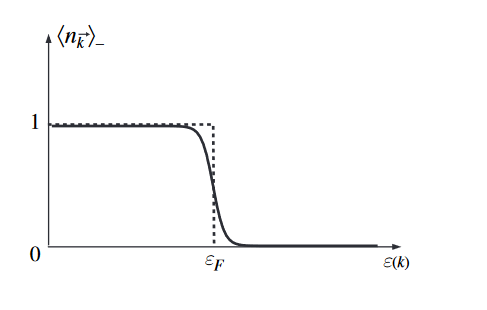
\includegraphics[scale=0.8]{figures/fermi_dist.png}
\end{figure}


\noindent For an ideal Fermi gas, 
\begin{align*}
	\mathcal{E}(\vec{k}) = \f{\hbar^2 k^2}{2m} \implies \mathcal{E}_F \coloneqq \f{\hbar^2 k_F^2}{2m}
\end{align*}
where $k_F$ is the \textbf{Fermi wavenumber}. The Fermi wavenumber $k_F$ can be computed from the number density as:
\begin{align*}
	n = \int_{k < k_F} g \times  \f{d^3 \vec{k}}{(2\pi)^3} =  g\int_{k< k_F} 4\pi k^2 \f{dk}{(2\pi)^3} = \f{g}{6\pi^2}k_F^3.
\end{align*}
So,
\begin{align*}
	\boxed{k_F = \lp \f{6\pi^2 n}{g} \rp^{1/3} \implies \mathcal{E}_F = \f{\hbar^2}{2m} \lp \f{6\pi^2 n}{g} \rp^{2/3}}
\end{align*}

To extract thermodynamics properties of the degenerate Fermi gas in three dimensions (untrapped), we consider the high-$z$ limit of $f_m^-(z)$. Again, Chapter 7 of \cite{kardar2007statistical} shows the details of the various expansions. The result is the \textbf{Sommerfeld expansion}:
\begin{align*}
	\lim_{z\to \infty} f_m^-(z) = \f{(\ln z)^m}{m!} \lb 1 + \f{\pi^2}{6}  \f{m(m-1)}{(\ln z)^2} + \f{7\pi^4}{360} \f{m(m-1)(m-2)(m-3)}{(\ln z)^4} + \dots \rb
\end{align*} 
From the $n_\eta$ equation in the previous section, we find that in the degenerate limit, the density and chemical potential are related by 
\begin{align*}
	\f{n\lambda^3}{g} = f_{3/2}^{-}(z) = \f{(\ln z)^{3/2} }{(3/2)!}\lb 1 + \f{\pi^2}{6}\f{3}{2}\f{1}{2}(\ln z)^{-2}  + \dots \rb \gg 1
\end{align*}

\begin{figure}[!htb]
	\centering
	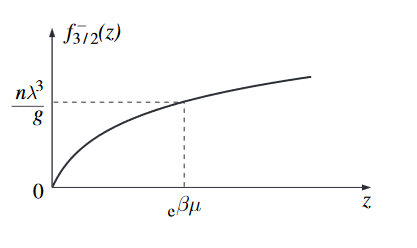
\includegraphics[scale=0.8]{figures/chem_pot.png}
\end{figure}

To lowest order, we have
\begin{align*}
	\lim_{T\to 0} \ln z = \lp \f{3}{4\sqrt{\pi}} \f{n\lambda^3}{g} \rp^{2/3} = \f{\be \hbar^2}{2m} \lp \f{6\pi^2 n}{g} \rp^{2/3} = \be \mathcal{E}_F \implies \lim_{T\to 0} \mu = \mathcal{E}_F
\end{align*}
which is what we found earlier by looking at the mean occupation number for fermions. \\



At finite but small temperatures, we have corrections:
\begin{align*}
	\ln z \approx \be \mathcal{E}_F \lb 1 - \f{\pi^2}{12} \lp \f{k_B T}{\mathcal{E}_F} \rp^2 + \dots \rb
\end{align*}

\begin{figure}[!htb]
	\centering
	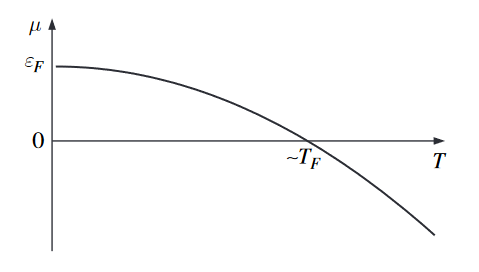
\includegraphics[scale=0.8]{figures/chem_pot_v_T.png}
\end{figure}

We see that the chemical potential $\mu = k_B T \ln z$ is positive at low temperature and negative at high temperature. It changes sign at $T \sim T_F = \mathcal{E}_F/k_B$. \\


Using a similar approach, one finds the low-temperature expansion for pressure:
\begin{align*}
	\be P = \be P_F\lb 1 + \f{5}{12}\pi^2 \lp \f{k_B T}{\mathcal{E}_F} \rp^2 + \dots \rb, \quad\quad \boxed{P_F = \f{2}{5}n \mathcal{E}_F}
\end{align*}
Here $P_F$ is the \textbf{fermi pressure}. Note that the fermi gas at zero temperature has nonzero pressure and internal energy, unlike its classical counterpart. 

\begin{figure}[!htb]
	\centering
	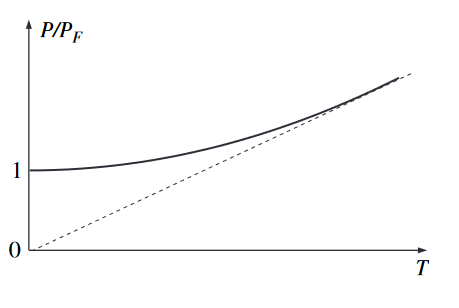
\includegraphics[scale=0.8]{figures/fermi_pressure.png}
\end{figure}

The internal energy (density) is obtained from the third equation in the previous section: 
\begin{align*}
	\boxed{\epsilon = \f{E}{V} = \f{3}{2}P = \f{3}{5}nk_B T_F \lb 1 + \f{5}{12}\pi^2 \lp \f{k_B T}{\mathcal{E}_F} \rp^2 + \dots \rb}
\end{align*}

From here, one finds the low-temperature heat capacity:
\begin{align*}
	C_V = \f{dE}{dT} = \f{\pi^2}{2}Nk_B \lp \f{T}{T_F} \rp + \mathcal{O}\lp \f{T}{T_F}  \rp^3
\end{align*}

\begin{figure}[!htb]
	\centering
	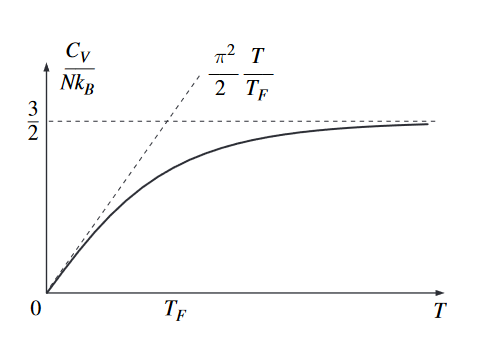
\includegraphics[scale=0.8]{figures/heat_cap.png}
\end{figure}


Note: the linear scaling of $C_V$ as $T\to 0$ is a general feature of a fermi gas and is valid in all dimensions. The physical interpretation is as follows: At small temperatures, all single-particle states are occupied. As a result, only particles within a distance of about $k_B T$ of the fermi energy can be thermally excited. This represents only a small fraction $(T/T_F)$ of the fermions. Each excited particle gains $k_B T$, leading to a change in $E$ of $k_B T N (T/T_F)$. So $C_V \propto dE/dT \sim N k_BT/T_F$ which is linear in $T$. This conclusion is also \textbf{valid for interacting fermi gases}. 



\section{Ideal Fermi gas in a harmonic trap}

See next chapter. This section is more naturally treated in conjunction with a number of related topics.


\chapter{Interacting Fermi Gas}


\section{Hyperfine Structure}

\section{Collisional Properties}


\section{Cooling and Trapping techniques}


\section{RF Spectroscopy}


\section{Feshbach resonance}

This section is adapted from \cite{campbellfeshbach} and \cite{ketterle2008making}.


\subsection{Scattering theory}

\subsection{Application: Spherical Well Model}

\subsection{Application: Coupled Square Well Model}

\subsection{An intuitive picture}




\section{Analysis of density distributions}













\chapter{Strongly Interacting Fermi Gas}


\bibliographystyle{abbrv} 
\bibliography{BUI_Fermi_refs}% Produces the bibliography via BibTeX.




	
	
\end{document}